\documentclass[11pt]{article}

\usepackage[margin=1in]{geometry}
\usepackage[utf8]{inputenc}
\usepackage{amsmath}
\usepackage{bigints}
\usepackage{graphicx}
\usepackage{float}
\usepackage{subfig}
\usepackage{hyperref}

\pagestyle{plain}

\title{Devoir 1 - \textbf{LINMA1170}}
\author{Hugo Vandermosten - \textbf{25741900}}
\date{2022}

\begin{document}


% L'ensemble des images utilisées dans ce rapport, le code complet et les images produites pour la création de la petite vidéo de simulation sont disponibles sur le git suivant : https://github.com/dsfaqfq/LINMA1170-devoir1.git

\maketitle

\section{Résolution du problème}

\subsection{Construction du système}

Le système à résoudre pour chaque pas de temps est décrit par $M^2 + 8$ équations et $M^2 + 8$ inconnues. Les $M^2$ premières inconnues sont les évaluations du champ scalaire $a(x,y,t)$ aux points étudiés, donc $a_{i,j}(t) \approx a(\Delta x*i, \Delta x*j, t)$  où  $i,j \in \{ 1,...,M \}$. Les huit dernières inconnues sont les chutes de tension $U_{pq}$ suivies du courant $I_{pq}$ des quatre spires $S_{pq}$ où $p,q = 1,2$. \\
Dans ma solution, le vecteur $x$ est donc le suivant : 
\begin{center}
    $x =$
    $\left(
    \begin{smallmatrix}
       a_{1,1} & a_{2,1} & \hdots & a_{M,1} & a_{1,2} & \hdots & a_{M,M} & U_{11} & \hdots & U_{22} & I_{11} & \hdots & I_{22}
    \end{smallmatrix}
    \right)$
\end{center}

\subsubsection{Équations liées aux dérivées partielles}

Les $M^2$ premières équations retranscrites dans les $M^2$ premières lignes de la matrice $A$ et du vecteur $b$ sont celles liées aux dérivées partielles de $a$. Celles-ci ont été linéarisées à l'aide des différences finies, ce qui donne le résultat suivant :

\begin{center}
    $\frac{1}{\mu_0} \left( \frac{\partial^2a}{\partial x^2} + \frac{\partial^2a}{\partial y^2} \right) + j = 0$ \\
    $\Longrightarrow \frac{1}{\mu_0} \left(\frac{a_{i-1,j} + a_{i,j-1} - 4a_{i,j} + a_{i+1,j} + a_{i,j+1}}{ \left(\Delta x\right)^2} \right) + j = 0 $ 
    $$ \textrm{où }
    j = \left\{
        \begin{array}{ll}
            \sigma \left( - \frac{\partial a}{\partial t} - \mbox{grad}u\right) \approx \sigma \left(\frac{a_{i,j}^{t-1} - a_{i,j}^t}{\Delta t} + \frac{U_{pq}}{L_z} \right) & \mbox{si } a_{i,j} \mbox{ est dans la spire } S_{pq} \\
            0 & \mbox{sinon.}
        \end{array}
    \right.
    $$
\end{center}

\subsubsection{Équations liées au courant dans les spires}
Dans la construction du système matriciel, les 4 équations linéarisées suivantes sont celles-ci :
\begin{center}
    $I_{pq} = \bigintss_{S_{pq}}j~dS{pq} = \sigma\bigintss_{S_{pq}} \left(-\frac{\partial a}{\partial t} + \frac{U_{pq}}{L_z} \right)~dS{pq}$ \\
    $\Longrightarrow I_{pq} \approx \sigma \underset{k\in S_{pq}}{\sum} \left< \frac{a_{i,j}^{t-1} - a_{i,j}^t}{\Delta t} + \frac{U_{pq}}{L_z}\right>_k \left(\Delta x\right)^2 $ \\
\end{center}
Dans cette dernière équation, on peut simplifier l'expression en remarquant que pour sommer \\ $\left<\frac{a_{i,j}^{t-1} - a_{i,j}^t}{\Delta t}\right>\left(\Delta x\right)^2$ pour chaque cellule carrée $k$ inclue dans le maillage de la spire $S_{pq}$, on peut le réécrire comme suit :
\begin{center}
    $\underset{k\in S_{pq}}{\sum} \left< \frac{a_{i,j}^{t-1} - a_{i,j}^t}{\Delta t}\right>_k \left(\Delta x\right)^2= \underset{k\in S_{pq}}{\sum} \frac{n_{i,j,k}}{4}\left(\frac{ a_{i,j}^{t-1} - a_{i,j}^t}{\Delta t} \right)\left(\Delta x\right)^2$
\end{center}
Où $n_{i,j,k} $ est le nombre de cellules carrées $k \in S_{pq}$ avec lesquelles le point $(\Delta x*i,\Delta x*j)$ coïncide.\\
De plus, comme $U_{pq}$ ne dépend pas de la position du carré $k$, on peut écrire :
\begin{center}
    $\underset{k\in S_{pq}}{\sum} \left< \frac{a_{i,j}^{t-1} - a_{i,j}^t}{\Delta t}\right>_k\left(\Delta x\right)^2 = U_{pq} * A_S$
\end{center}
Où $A_S$ est la surface d'une coupe d'une spire.
\subsubsection{Équations liées au circruit}
Les équations liées au circuit sont très simple et donc complètement développées dans l'énoncé du devoir, elles sont représentées dans les 4 dernières lignes de la matrice $A$ du système d'équations linéaires.


\subsection{Résolution itérative du système}

\subsubsection{Factorisation LU avec pivot}

Pour éviter tout problème de division par $0$ ou par un nombre trop petit (lié à des erreurs d'arrondis ou autre), il est bien plus prudent, pour la factorisation LU, d'utiliser la méthode avec pivot vue en cours. L'implémentation utilisée dans la résolution du devoir est celle décrite dans le cours et qui a été implémentée lors du TP3.

\subsubsection{calculs à effectuer à chaque itération}

Pour résoudre le système à chaque itération, il est nécessaire d'effectuer 3 actions pour chaque pas de temps.
\begin{itemize}
    \item Mise à jour du vecteur $b$ à l'aide des résultats (vecteur $x$) de l'itération précédente et du temps $t$.
    \item Application d'une "forward substitution" (en prenant en compte les pivots utilisés).
    \item Application d'une "backward substitution".
    
\end{itemize}

\section{Visualisation des lignes de champ magnétique}

La visualisation des lignes du champ magnétique sur le domaine étudié peut se faire facilement en récupérant les valeurs utiles dans $x$ à chaque itération. L'utilisation de la librairie matplotlib de Python permet de facilement visualiser ces résultats. Et en les affichant les uns à la suite des autres, on peut obtenir une représentation assez visuelle du champ magnétique étudié avec des pas de temps et de distance suffisamment petits. Une visualisation réalisée pour les paramètres $\{M,Mt,f\} = \{39,90,500\}$ est disponible \href{https://youtu.be/3ytU4as6qUQ}{\textbf{ici}}.

\section{Le phénomène de fill-in}
\subsection{Explication du phénomène}
Le fill-in d'une matrice est le nombre d'éléments qui passent d'une valeur nulle à une valeur non-nulle lors de l'exécution d'un algorithme sur celle-ci. Lors d'une factorisation LU, le nombre d'éléments non-nuls de la matrice factorisée est toujours supérieur à celui de la matrice initiale. Cela s'explique par le fait que, à chaque itération de l'algorithme, on a $C = C + vu^T$ où $C$ est le masque booléen de la matrice étudiée. Cela signifie que les entrées $C_{ij}$ où $v_i$ et $u_j$ sont à "\textbf{True}" prennent également la valeur "\textbf{True}". L'ordre des lignes et des colonnes de la matrice étudiée est donc extrêmement importants si on veut garder une matrice factorisée la plus creuse possible.
Par exemple, dans l'exemple suivant, on peut passer de la création d'une matrice quasiment pleine à un fill-in nul en inversant deux colonnes.
\begin{center}
    $
    \begin{pmatrix}
       1 & 0 & 0 & 0 & 0 & 0 \\
       2 & 1 & 0 & 0 & 0 & 0 \\
       3 & 0 & 1 & 0 & 0 & 0 \\
       4 & 0 & 0 & 1 & 0 & 0 \\
       5 & 0 & 0 & 0 & 1 & 0 \\
       6 & 2 & 3 & 4 & 5 & 6 \\
    \end{pmatrix}
    ~~
    \underset{\textrm{LU (avec pivot)}}{\Longrightarrow}
    ~~~
    \begin{pmatrix}
       6   & 2    & 3      & 4       & 5    & 6 \\
       1/6 & -1/3 & -1/2   & -2/3    & -5/6 & -1 \\
       1/3 & -1   & -3/2   & -2      & -5/2 & -3 \\
       1/2 & 3    & -2/3   & 4/3     & -5/3 & -2 \\
       2/3 & 4    & 0      & -3/4    & -5/4 & -3/2 \\
       5/6 & 5    & -3e-16 & 1.1e-16 & -8   & -6/5 \\
    \end{pmatrix}
    $ \\
    $
    \begin{pmatrix}
       0 & 0 & 0 & 0 & 0 & 1 \\
       0 & 1 & 0 & 0 & 0 & 2 \\
       0 & 0 & 1 & 0 & 0 & 3 \\
       0 & 0 & 0 & 1 & 0 & 4 \\
       0 & 0 & 0 & 0 & 1 & 5 \\
       6 & 2 & 3 & 4 & 5 & 6 \\
    \end{pmatrix}
    ~~
    \underset{\textrm{LU (avec pivot)}}{\Longrightarrow}
    ~~~
    \begin{pmatrix}
       6 & 2 & 3 & 4 & 5 & 6 \\
       0 & 1 & 0 & 0 & 0 & 2 \\
       0 & 0 & 1 & 0 & 0 & 3 \\
       0 & 0 & 0 & 1 & 0 & 4 \\
       0 & 0 & 0 & 0 & 1 & 5 \\
       0 & 0 & 0 & 0 & 0 & 1 \\
    \end{pmatrix}
    $

\end{center}
De plus, on peut observer ici via l'apparition de termes comme $1.1e-16$ que l'utilisation successive de pivots peut faire apparaître des petites erreurs d'arrondis dans la factorisation.

\subsection{le fill-in dans le devoir}

Avec la construction de la matrice $A$ décrite précédemment, on observe un fill-in raisonnable, représenté sur les images ci-dessous pour des paramètres de base. Cependant, il est intéressant de noter qu'en changeant l'ordre des équations pour que les 8 premières lignes correspondent aux équations liées au courant et au circuit, la factorisation LU avec pivot fait déjà augmenter le nombre de valeurs non-nulles dans le résultat.

\begin{figure}[H]
    \centering
    \subfloat[\centering ordre original]{{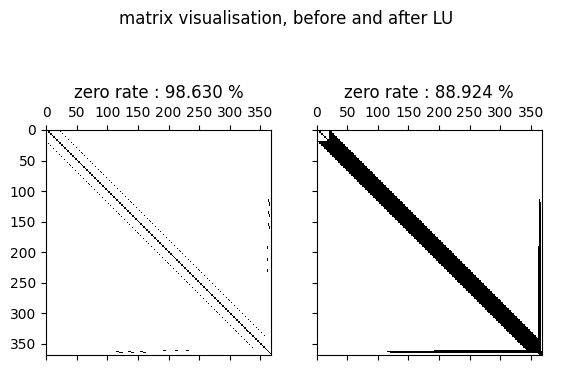
\includegraphics[width=0.4\textwidth]{plot_matrix/M19.png} }}
    \qquad
    \subfloat[\centering ordre modifié]{{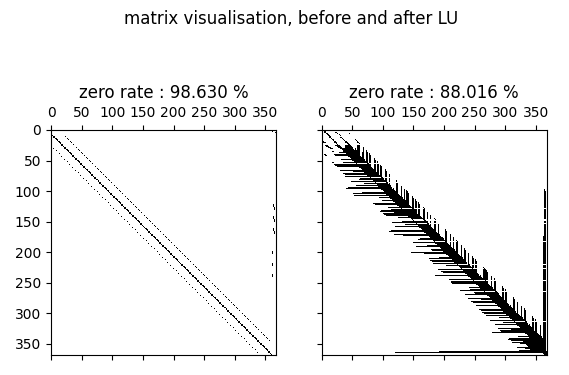
\includegraphics[width=0.4\textwidth]{plot_matrix/M19_Modified.png} }}
    \caption{Visualisation des valeurs non-nulles de $A ~ \big(\{M, Mt, f\} = \{19, 8, 1\} \big) $ }
    \label{fig:example}
\end{figure}

\section{Comparaison et discussion des résultats en fonction de $M$ et $Mt$}

L'utilisation de valeurs plus grandes pour les paramètres $M$ et $Mt$ implique une discrétisation du problème plus importante et donc des pas (de temps pour $Mt$ et de distance pour $M$) plus petits. L'utilisation de pas plus petits pour la discrétisation augmente donc la précision de la solution, car les erreurs que la linéarisation du système provoque sont des fonctions (croissantes évidemment) dépendantes de ceux-ci. Par exemple, la discrétisation de l'opérateur Laplacien est en $\mathcal{O}((\Delta x)^2)$. De plus, si on regarde les puissances entrantes et sortantes du mécanisme à tous les pas de temps étudiés (sur deux périodes), on observe un affinage clair des résultats quand $M$ et $Mt$ augmentent. Il est également important de noter que les équations ne gardent du sens que si $M+1$ est un multiple de $20$ (le maillage coïncide avec les spires.).

\begin{figure}[H]
    \centering
    \subfloat[\centering $M = 19, Mt = 8$]{{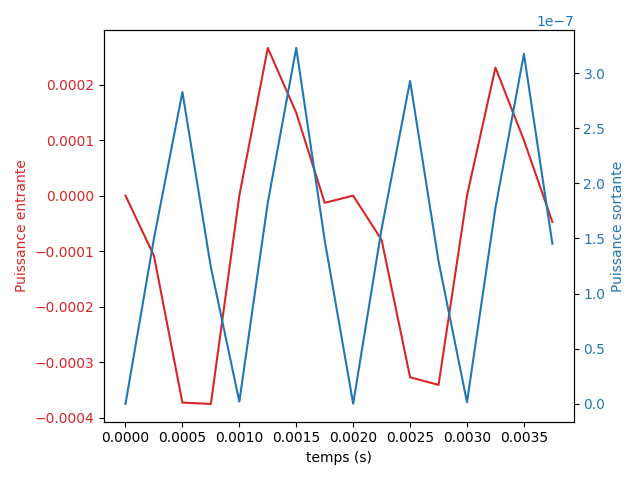
\includegraphics[width=0.25\textwidth]{plot_power/M19Mt8.png} }}
    \subfloat[\centering $M = 19, Mt = 30$]{{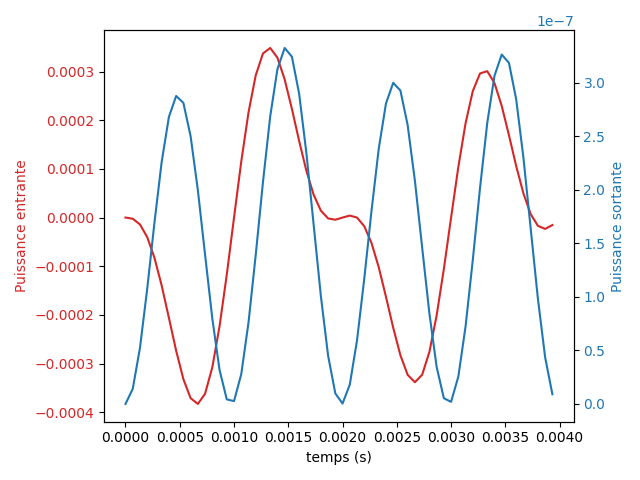
\includegraphics[width=0.25\textwidth]{plot_power/M19Mt30.png} }}
    \subfloat[\centering $M = 19, Mt = 90$]{{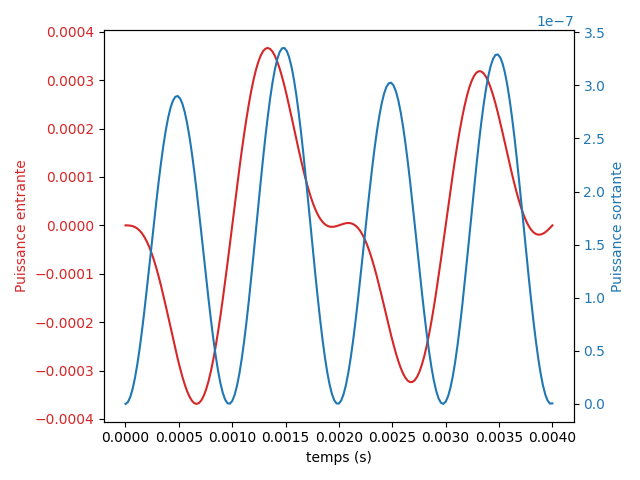
\includegraphics[width=0.25\textwidth]{plot_power/M19Mt90.png} }}
    \vspace{-4mm}
    \subfloat[\centering $M = 39, Mt = 8$]{{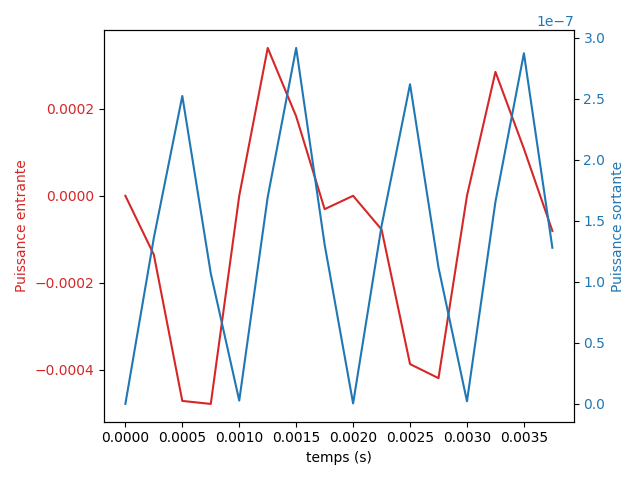
\includegraphics[width=0.25\textwidth]{plot_power/M39Mt8.png} }}
    \subfloat[\centering $M = 39, Mt = 30$]{{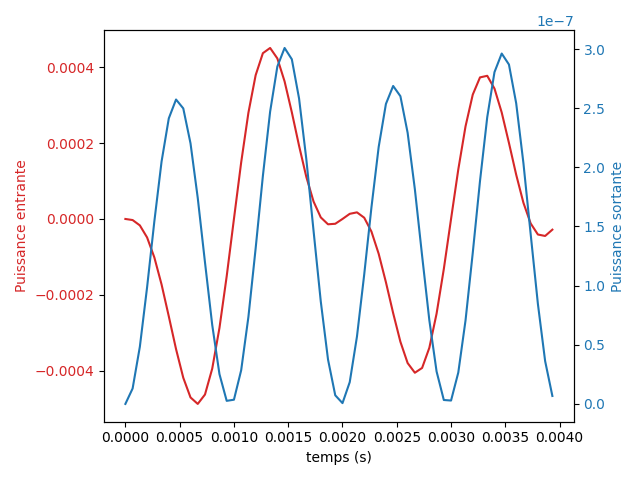
\includegraphics[width=0.25\textwidth]{plot_power/M39Mt30.png} }}
    \subfloat[\centering $M = 39, Mt = 90$]{{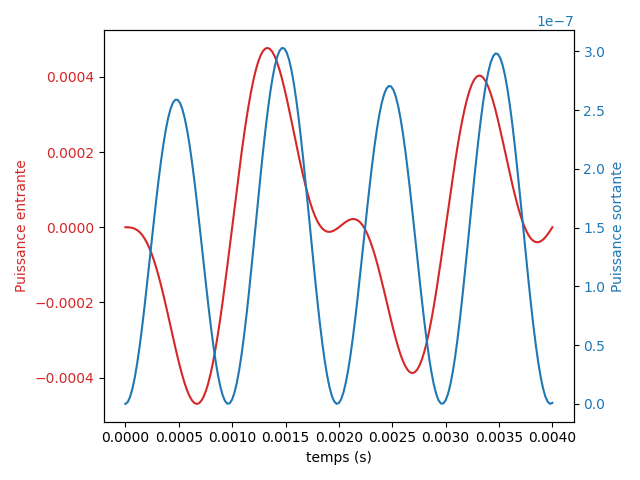
\includegraphics[width=0.25\textwidth]{plot_power/M39Mt90.png} }}
    \vspace{-4mm}
    \subfloat[\centering $M = 59, Mt = 8$]{{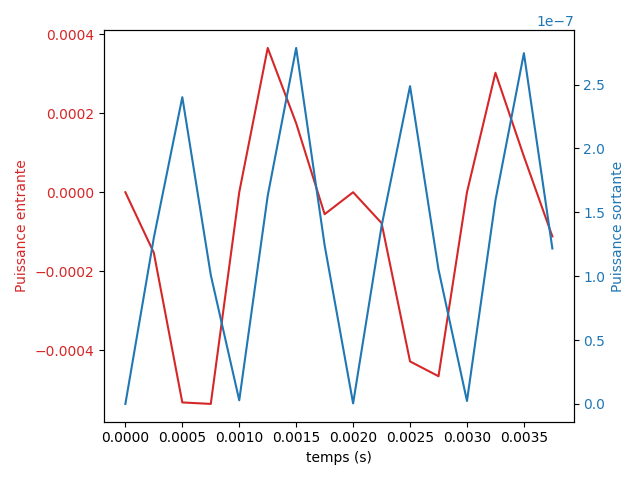
\includegraphics[width=0.25\textwidth]{plot_power/M59Mt8.png} }}
    \subfloat[\centering $M = 59, Mt = 30$]{{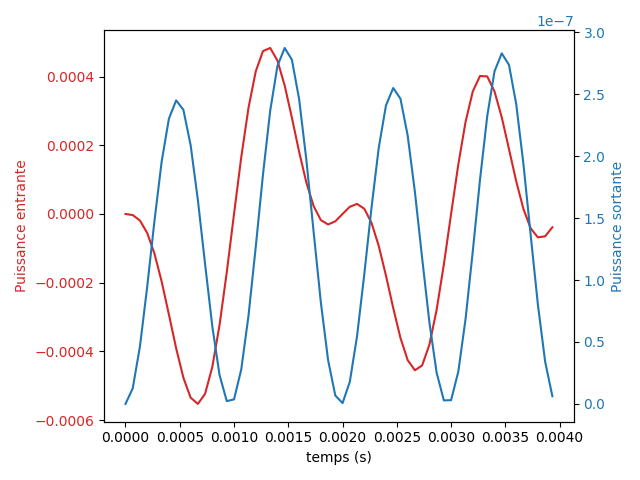
\includegraphics[width=0.25\textwidth]{plot_power/M59Mt30.png} }}
    \subfloat[\centering $M = 59, Mt = 90$]{{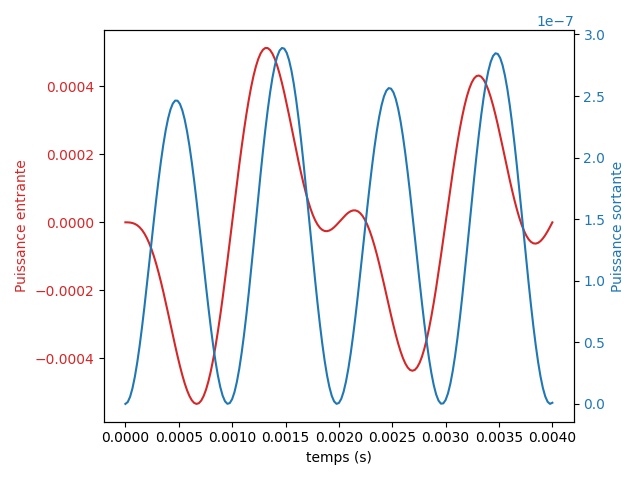
\includegraphics[width=0.25\textwidth]{plot_power/M59Mt90.png} }}


    \caption{Comparaison des puissances entrantes et sortantes en fonction de $M$ et $Mt$ }
    \label{fig:example}
    
\end{figure}

\section{Proposition d'accélération de la factorisation LU}

La matrice $A$ étant une matrice creuse (encore plus si $M$ augmente), il existe de nombreuses manières d'accélérer sa factorisation LU. On peut par exemple utiliser une autre manière de l'enregistrer comme le \textit{Sparse Storage Schemes} (CSR) et adapter l'algorithme en fonction. Une autre manière d'accélérer l'algorithme serait de réordonner la matrice A pour limiter le phénomène de fill-in et le nombre de calculs nécessaires. Le problème d'optimisation du fill-in étant NP-complet, il n'est pas envisageable de trouver une solution parfaite, mais on peut tout de même, par exemple, utiliser le \textit{Reverse Cuthill-Mckee algorithm} pour essayer de réduire le fill-in.

\end{document}

\end{document}
